
\section{Post-{N}ewtonian approximations}
\label{sec:PNWaveforms}

\subsection{Effective One-Body}
\label{ssec:EOB}

\section{Numerical Relativity}
\label{sec:NRWaveforms}

\section{Hybrid waveforms}
\label{sec:HybridWaveforms}


\iffalse
% Taken from Boyle et. al, left here as a reminder of
% material to cover.

\subsection{Post-{N}ewtonian template}
\label{sec:PNWaveforms}

Searches for gravitational waves in LIGO and Virgo use a
post-Newtonian waveform known
as\textit{TaylorF2}~\cite{Abbott:2008}. This is a frequency-domain
waveform obtained via the stationary-phase
approximation~\cite{CutlerFlanagan1994}, which assumes that the
frequency-domain amplitude is simply proportional to $f^{-7/6}$ (the
lowest-order behavior), while its phasing is given by the phase of the
time-domain waveform, as a function of frequency.  For a binary
consisting of masses $m_{1}$ and $m_{2}$, located at an ``effective''
distance $\deff$, we have
\begin{equation}
  \tilde{h}(f; M, \eta, f_{c}) =
  % \left(\frac{5\pi}{24}\right)^{1/2}
  % \left(\frac{G{\mathcal{M}}}{c^3}\right)
  % \left(\frac{G{\mathcal{M}}}{c^2\deff}\right)
  % \left(\frac{G{\mathcal{M}}}{c^3}\pi f\right)^{-7/6}
  % \e^{i\Psi(f;M,\eta)}
  \Theta(f_c - f)\, \left(\frac{\unit[1]{Mpc}}{\deff}\right)\,
  {\mathcal{A}}_{\unit[1]{Mpc}}(M,\eta)\, f^{-7/6}\,
  \e^{i\varphi(f;M,\eta)}\ ,
  \label{e:waveform}
\end{equation}
where
\begin{eqnarray} {\mathcal{A}}_{\unit[1]{Mpc}}(M,\eta) &= &
  \left(\frac{5\pi}{24}\right)^{1/2}
  \left(\frac{\G \MSun/\c^2}{\unit[1]{Mpc}}\right) \times \nonumber \\
  &\quad & \times \left(\frac{\pi \G \MSun}{\c^3}\right)^{-1/6}
  \left(\frac{\eta}{\MSun}\right)^{1/2}
  \left(\frac{M}{\MSun}\right)^{1/3}\ ,
\end{eqnarray}
and the phasing $\varphi$ of the frequency-domain waveform is given to
3.5pN accuracy by the formula~\cite{Blanchet.2002,Blanchet.2004}
\begin{eqnarray}
  \varphi(f;M,\eta) &=& 2\pi ft_0-2\phi_0-\pi/4 \nonumber \\
  &&+ \frac{3}{128\eta}\Bigg[v^{-5}
  +\left(\frac{3715}{756}+\frac{55}{9}\eta\right)v^{-3}-16\pi v^{-2} \nonumber \\
  &&+ \left(\frac{15\,293\,365}{508\,032}+\frac{27\,145}{504}\eta
    +\frac{3085}{72}\eta^2\right)v^{-1} \nonumber \\
  &&+ \pi \left[ \frac{38\,645}{756} -
    \frac{65}{9}\eta \right] \left[1 + 3
    \ln\left(\frac{v}{v_0}\right) \right] \nonumber \\
  &&+ \left[\frac{11\,583\,231\,236\,531}{4\,694\,215\,680}
    - \frac{640}{3} \pi^2 - \frac{6\,848}{21} \gamma \right] v \nonumber \\
  &&+ \bigg[\left(-\frac{15\,335\,597\,827}{3\,048\,192} +
    \frac{2\,255}{12} \pi^2 - \frac{47\,324.0}{63.0} -
    \frac{794\,8}{9}\right) \eta \nonumber \\
  & & \qquad + \frac{76\,055}{1\,728} \eta^2
  - \frac{127\,825}{1\,296} \eta^3 \bigg] v \nonumber \\ 
  &&+ \pi
  \left[ \frac{77\,096\,675}{254\,016} + \frac{378\,515}{1\,512}
    \eta - \frac{74\,045}{756} \eta^2 \right] v^2\Bigg]\ .
\end{eqnarray}
where $v = \left(\frac{\G M}{\c^3}\pi f\right)^{1/3}$, $M = m_{1} +
m_{2}$ and $\eta =m_1 m_2/(m_1+m_2)^2$.


The overall frequency scale is set by the total mass $M$, as can be
seen by observing that each occurrence of $f$ is accompanied by a
factor of $M$.\footnote{The term $2\pi f t_{0}$ might be rewritten as
  $2\pi Mf \times t_{0}/M$.  This term accounts for a time offset
  altering the phase of the Fourier transform.}  %
Thus, going to a higher-mass system shifts the waveform to lower
frequencies.  On the other hand, to first order, the timescale for the
rate of change of the frequency is given by the \textit{chirp mass}:
\begin{equation}
  \label{eq:ChirpMass}
  \mathcal{M} \equiv \left( \frac{m_{1}^{3}\, m_{2}^{3}} {m_{1} +
      m_{2}} \right)^{1/5} = M\, \eta^{3/5}\ .
\end{equation}
Clearly, the total mass and chirp mass give us two very different
handles on the behavior of the waveform.  These two handles will be
important when we try to match the template to our waveform in regions
where the post-Newtonian and stationary-phase approximations are poor.
This is typically the case for high-mass systems, which only enter the
detector band late in the inspiral.  In this case, we can still obtain
a high match, at the cost of using templates with the wrong values of
$M$ and $\eta$.

We also note that physical binary systems are restricted to $0 < \eta
\leq 1/4$.  However, for higher values of $\eta$, the formulas shown
above still give plausible waveforms; in fact, in some cases these
templates match the true waveform better than any physical template.
We will explore the implications of allowing unphysical values for
$\eta$ in searches over the templates in
Sec.~\ref{sec:UnrestrictedEta}.

Note the Heaviside function in Eq.~\eqref{e:waveform}.  This contains
a cutoff frequency $f_{c}$ which is used to ensure that the template
does not extend to frequencies much greater than the frequencies
contained in the expected signal.  This is essentially a third
parameter for the template waveform, and will be searched over.  See
Sec.~\ref{sec:EffectOfUpperFreqCutoff} for a discussion of strategies
for optimizing detection by changing this cutoff.

Frequencies which are often used to characterize coalescing binary
black holes are: (i) the frequency at the innermost stable circular
orbit (ISCO), $r=6 M$, around a single Schwarzschild black hole with
the total mass of the binary system; (ii) the frequency at the light
ring, $r=3.0/M$, around a single Schwarzschild black hole with the
total mass of the binary system; (iii) the ringdown frequency of the
final black hole, which depends on both its spin and mass; and (iv) an
``effective ringdown,'' $f_{\mathrm{ERD}} \equiv 1.07\,
f_{\mathrm{Ringdown}}$ defined in~\cite{Pan2007}.


Current searches use 2pN stationary-phase approximation (SPA)
\textit{TaylorF2} templates~\cite{Abbott:2008}.  It has previously
been shown that such waveforms provide acceptable detection templates
for binary neutron stars and sub-solar mass black
holes~\cite{Droz:1999qx}, but not necessarily for higher-mass black
holes.  This is an issue we will investigate below by testing 2pN and
3.5pN templates.



\section{NR}
Optimal searches for gravitational waves use matched filtering, which
requires accurate knowledge of the waveform~\cite{thorne.k:1987}.
Previous searches in LIGO data have used post-Newtonian and
phenomenological templates to search for the coalescence of black-hole
binaries~\cite{Abbott:2005pf,Abbott:2007xi,Abbott:2008}. Over the last
several years numerical relativity has made remarkable breakthroughs
in simulating the late inspiral, merger and ringdown of black-hole
binaries. The computational cost of these simulations is high,
however, making it impractical to use them directly as template
waveforms for use in a matched-filter search. It has been shown that
there is good agreement between the waveforms generated by numerical
relativity with analytic post-Newtonian waveforms to within just a few
orbits of merger~\cite{Buonanno-Cook-Pretorius:2007, Baker2006d,
  Pan2007, Buonanno2007, Hannam2007, Boyle2007, Gopakumar:2007vh,
  Hannam2007c, Boyle2008a, Mroue2008, Hinder2008b}.


\subsection{Hybrid waveform}
\label{sec:HybridWaveform} %
Numerical simulations cannot simulate a very large portion of the
inspiral of a black-hole binary system.  Indeed, the longest such
simulation currently in the literature is the one used here---which
extends over just 32 gravitational wave cycles before merger.
Fortunately, this is the only stage in which simulations are needed.
It has been shown previously~\cite{Boyle2007} that the
\textit{TaylorT4} waveform with 3.5-pN phase and 3.0-pN amplitude
matches the early part of this simulation to very high accuracy.  We
generate a \textit{TaylorT4} waveform of over 8000 gravitational wave
cycles ($t \sim 1.2\times 10^{6}M$, starting at $M f=0.004$), and
transition between the two to create a hybrid.  This long waveform is
sufficient to ensure that---even for the lowest-mass systems we will
consider---the waveform begins well before it enters the frequency
band of interest to LIGO.

We begin with $\Psi_4$ data, which will later be integrated to obtain
$h$.  Following Ref.~\cite{Boyle2008a}, we match the numerical
waveform to the pN waveform by adjusting the time and phase offsets of
the pN waveform to minimize the quantity
\begin{equation}
  \label{eq:MatchingChiSquared}
  \Xi(\Delta t, \Delta \phi) = \int_{t_{1}}^{t_{2}}\, \left[
    \phi_{\NR}(t) - \phi_{\pN}(t - \Delta t) - \Delta \phi
  \right]^{2}\, d t \ .
\end{equation}
Here, we choose $t_{1}=900\,M$ and $t_{2}=1730\,M$, which is closer to
the beginning of the waveform than in the previous paper.  This
particular interval is chosen to begin and end at troughs of the small
oscillations due to the residual eccentricity $e\sim 5\times 10^{-5}$
in our numerical waveform.  Taking a range from trough to trough or
peak to peak---rather than node to node, for example---of the
eccentricity effects minimizes their influence on the matching.  The
eccentricity oscillations can be seen more easily after low-pass
filtering the waveform, though we find filtering to be unnecessary for
this paper.  The junk radiation apparent in the waveform as shown here
has no effect on the resulting match---as we have verified by
filtering, and redoing the match.  Because the final waveform will
incorporate no numerical data before $t_{1}$ and very little
immediately thereafter (as explained below), the junk radiation will
have no effect on any of our results---as we have also explicitly
verified.  In particular, by integrating $\Psi_{4}$ to obtain $h$, we
will effectively smooth the junk radiation.

%%%%%%%%%%%%%%%%%%%%%%%%%%%%%%%%%%%%%%%%%%%%%%%%%%%%%%%%%%%%%%%%%%%%%%
\begin{figure}
  \begin{center}
    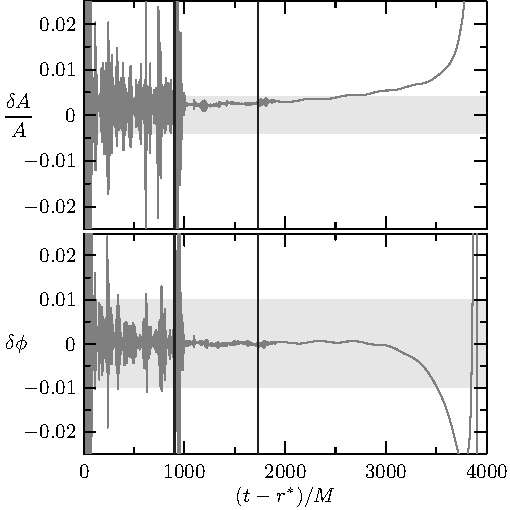
\includegraphics[width=0.55\linewidth]{figures/comparison/PlotDifferences}
  \end{center}
  \caption{Amplitude and phase differences between the numerical and
    post-Newtonian waveforms, $\Psi_4$, that are blended to create the
    hybrid waveform.  The vertical lines at $900M$ and $1730M$ denote
    the region over which matching and hybridization occur.  Note that
    the agreement is well within the numerical accuracy of the
    simulation, represented by the horizontal bands, throughout the
    matching region.  Also note that the phase difference is fairly
    flat for a significant period of time after the matching range,
    which indicates that the match is not sensitive to the particular
    range chosen for matching.}
  \label{fig:MatchingPhaseComparison}
\end{figure}%
%%%%%%%%%%%%%%%%%%%%%%%%%%%%%%%%%%%%%%%%%%%%%%%%%%%%%%%%%%%%%%%%%%%%%%
In Fig.~\ref{fig:MatchingPhaseComparison} we compare the phase of the
numerical and pN waveforms.  The quantities plotted are
\begin{eqnarray}
  \delta \phi & \equiv & \phi_{\pN} - \phi_{\NR}\ , \\
  \frac{\delta A}{A} & \equiv & \frac{A_{\pN} - A_{\NR}}{A_{\NR}}\ , 
\end{eqnarray}
shown over the interval on which both data sets exist.  The vertical
bars denote the matching region.  Note that the phase difference is
well within the accuracy of the simulation (about 0.01 radians,
represented by the horizontal band) over a range extending later than
the matching region.  Also, the difference between the two is fairly
flat, which implies that the match is not very sensitive to the region
chosen for matching.  Because of this, we expect that the phase
coherence between the early pN data and the late NR data will be
physically accurate to high precision.

The hybrid waveform is then constructed by blending the two matched
waveforms together according to
\begin{eqnarray}
  \label{eq:HybridWaveform}
  A_{\hyb}(t) &= & \tau(t)\, A_{\NR} + \left[ 1 - \tau(t) \right]\,
  A_{\pN}(t)\ , \\
  \phi_{\hyb}(t) &= & \tau(t)\, \phi_{\NR} + \left[ 1 - \tau(t)
  \right]\, \phi_{\pN}(t)\ .
\end{eqnarray}
The blending function $\tau$ is defined by

\begin{equation}
  \label{eq:BlendingFunction}
  \tau(t) = \left\{\begin{array}{ll}
      0 & \mathrm{if}\quad t<t_{1}  \\
      \frac{t-t_{1}}{t_{2}-t_{1}} & \mathrm{if}\quad t_{1} \leq t < t_{2} \\
      1 & \mathrm{if}\quad t_{2} \leq t
    \end{array} \right.
\end{equation}

The values of $t_{1}$ and $t_{2}$ are the same as those used for the
matching.  The amplitude discrepancy between the pN waveform and the
NR waveform over this interval is within numerical
uncertainty---roughly $0.4\%$.  As with the matching technique
(Eq.~(\ref{eq:MatchingChiSquared})), this method is similar to that of
Ref.~\cite{Ajith-Babak-Chen-etal:2007b}, but distinct, in that we
blend the phase and amplitude, rather than the real and imaginary
parts.  This leads to a smoothly blended waveform, shown in
Fig~\ref{fig:WaveformSnapshot}.
%%%%%%%%%%%%%%%%%%%%%%%%%%%%%%%%%%%%%%%%%%%%%%%%%%%%%%%%%%%%%%%%%%%%%%
\begin{figure}
  \begin{center}
    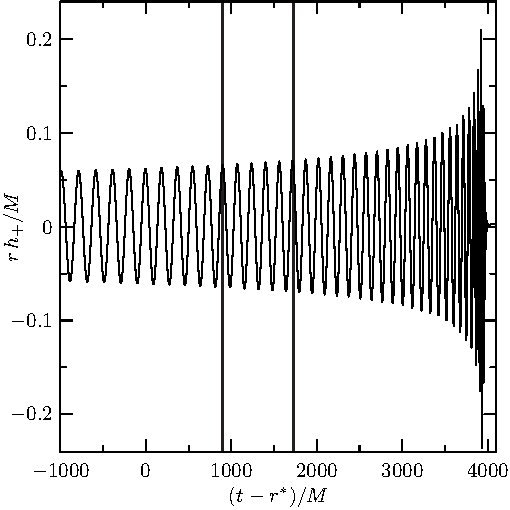
\includegraphics[width=0.55\linewidth]{figures/comparison/Waveform}
  \end{center}
  \caption{The last $t=5000\MSun$ of the hybrid waveform used in this
    analysis: the $h_{+}$ waveform seen by an observer on the positive
    $z$ axis.  The vertical lines denote the matching and
    hybridization region.  The $0$ on the time axis corresponds to the
    beginning of data from the numerical simulation.}
  \label{fig:WaveformSnapshot}
\end{figure}%
%%%%%%%%%%%%%%%%%%%%%%%%%%%%%%%%%%%%%%%%%%%%%%%%%%%%%%%%%%%%%%%%%%%%%%

Up to this point, the waveform has been $\Psi_{4}$ data.  With the
long waveform in hand, we numerically integrate twice to obtain $h$,
and set the four integration constants so that the final waveform has
zero average and first moment~\cite{Pfeiffer-Brown-etal:2007}.
Because of the very long duration of the waveforms, this gives a
reasonable result, which is only incorrect at very low
frequencies---lower than any frequency of interest to us.  We have
also checked that our results do not change when we effectively
integrate in the frequency domain by taking
\begin{equation}
  \label{eq:PsiFourIntegration}
  \tilde{h} = -\frac{\tilde{\Psi}_{4}}{4\,\pi\, f^{2}}\ ,
\end{equation}
which is the frequency-domain analog of the equation $\Psi_{4} =
\ddot{h}$.
\fi

